% !TEX root = ../main.tex
\section{Matematický fundament diferenciálních rovnic}
\label{sec:matematicky-fundament}

\blocktitle{Cíl kapitoly}
Vybudovat pevný teoretický rámec z funkcionální analýzy a teorie míry nezbytný pro pozdější formulaci slabých řešení, spektrálních metod a kvantových operátorů. Kapitola poskytne formální definice, motivaci a intuitivní příklady s důrazem na konstrukce používané ve studiích ODR, PDR i kvantových Hamiltoniánů.

\begin{intermezzo}
\textbf{Navázání na Kapitolu 1:} Zatímco Kapitola 1 nám představila diferenciální rovnice jako jazyk dynamických systémů, nyní potřebujeme vybudovat matematický aparát pro jejich rigorózní studium. Koncepty z Kapitoly 1 jako \hyperref[sec:uvod-diffeq]{fázové portréty}, \hyperref[sec:uvod-diffeq]{Picardova iterace} a \hyperref[sec:uvod-diffeq]{strukturální stabilita} nyní obdaříme přesným formalismem funkcionální analýzy. Konkrétně: Picardova iterace jako kontrakce v $C[a,b]$ a slabá formulace v $W^{1,2}$ rozšiřují naše možnosti pro existenci a regularitu řešení.
\end{intermezzo}

\spc

\subsection{Metrické a normované prostory}

\begin{scaffold}
\textbf{Co umíme:} Základní pojmy diferenciálních rovnic a jejich klasifikace z Kapitoly 1. \\
\textbf{Co se naučíme:} Jak měřit vzdálenosti a velikosti funkcí v abstraktních prostorech. \\
\textbf{K čemu to využijeme:} Pro studium konvergence aproximací a stability řešení ODR/PDR.
\end{scaffold}

\begin{motivation}
Abychom mohli rigorózně studovat konvergenci a stabilitu řešení diferenciálních rovnic, potřebujeme přesně definovat, jak měřit "vzdálenost" a "velikost" funkcí. Metrické a normované prostory poskytují tento fundamentální aparát.
\end{motivation}

\subsubsection{Základní definice a vlastnosti}

\begin{definition}[Metrický prostor]
Dvojice $(X,d)$, kde $X$ je množina a $d: X \times X \to \mathbb{R}$ je \emph{metrika} splňující:
\begin{enumerate}
\item $d(x,y) \geq 0$ a $d(x,y) = 0 \Leftrightarrow x = y$
\item $d(x,y) = d(y,x)$
\item $d(x,z) \leq d(x,y) + d(y,z)$
\end{enumerate}
\end{definition}

\begin{definition}[Normovaný prostor]
Dvojice $(X,\|\cdot\|)$, kde $X$ je vektorový prostor a $\|\cdot\|: X \to \mathbb{R}$ je \emph{norma} splňující:
\begin{enumerate}
\item $\|x\| \geq 0$ a $\|x\| = 0 \Leftrightarrow x = 0$
\item $\|\alpha x\| = |\alpha| \|x\|$
\item $\|x + y\| \leq \|x\| + \|y\|$
\end{enumerate}
\end{definition}

\begin{intuition}
Každá norma indukuje metriku $d(x,y) = \|x - y\|$, ale ne naopak. Norma měří "velikost", metrika "vzdálenost". V kontextu ODR: $\|f-g\|_\infty$ měří maximální odchylku mezi funkcemi na intervalu, což je klíčové pro analýzu stability řešení.
\end{intuition}

\subsubsection{Topologické aspekty a úplnost}

\begin{definition}[Metrická topologie]
Otevřené koule $B(x,r) = \{y \in X : d(x,y) < r\}$ generují topologii na metrickém prostoru.
\end{definition}

\begin{definition}[Cauchyho posloupnost]
Posloupnost $\{x_n\}$ v metrickém prostoru je \emph{Cauchyho}, jestliže pro každé $\epsilon > 0$ existuje $N$ takové, že $d(x_n, x_m) < \epsilon$ pro všechna $n,m > N$.
\end{definition}

\begin{definition}[Úplný prostor]
Metrický prostor je \emph{úplný}, jestliže každá Cauchyho posloupnost konverguje.
\end{definition}

\begin{definition}[Banachův prostor]
Úplný normovaný prostor.
\end{definition}

\begin{theorem}[O úplnosti]
Prostor $(C[a,b], \|\cdot\|_\infty)$ je Banachův prostor.
\end{theorem}

\begin{intuition}
Úplnost zajišťuje, že limity Cauchyho posloupností zůstávají v prostoru. Pro ODR: Picardova iterace $y_{n+1}(x) = y_0 + \int_{x_0}^x f(t,y_n(t))dt$ generuje Cauchyho posloupnost v $C[a,b]$, jejíž limita je řešením ODR. Kontrakční zobrazení v $\|\cdot\|_\infty$ normě zaručuje konvergenci této iterace.
\end{intuition}

\begin{keyinsight}
Úplnost je nezbytná pro konvergenci řad funkcí a iteračních metod. V ODR: Banachova věta o pevném bodě pro kontrakční zobrazení v úplných prostorech je základem konstruktivních důkazů existence řešení.
\end{keyinsight}

\subsubsection{Příklady a aplikace}

\begin{example}[Klasické prostory funkcí]
\mbox{}
\begin{itemize}
\item $(C[a,b], \|\cdot\|_\infty)$: spojité funkce s normou maxima
\item $(L^p(\Omega), \|\cdot\|_p)$: funkce s integrovatelnou $p$-tou mocninou
\item $(\ell^p, \|\cdot\|_p)$: posloupnosti s konvergentní řadou $p$-tých mocnin
\end{itemize}
\end{example}
    
    

\begin{application}
\begin{verbatim}
# Python: Picardova iterace pro y' = f(t,y), y(t0) = y0
def picard_iteration(f, t0, y0, t_span, n_iterations):
    t = np.linspace(t_span[0], t_span[1], 100)
    y = np.full_like(t, y0)
    for _ in range(n_iterations):
        y_new = y0 + cumtrapz(f(t[:-1], y[:-1]), t, initial=0)
        y = y_new
    return t, y
\end{verbatim}
Banachova věta o pevném bodě zaručuje konvergenci Picardovy iterace v úplných prostorech. Pro Lipschitzovskou funkci $f$ je zobrazení $T(y)(x) = y_0 + \int_{x_0}^x f(t,y(t))dt$ kontrakcí v $C[a,b]$ pro dostatečně malý interval, což zaručuje existenci a jednoznačnost řešení ODR.
\end{application}

\begin{summary}
\textbf{Klíčové koncepty:} Metrika, norma, úplnost, Banachův prostor. \\
\textbf{Hlavní výsledky:} $(C[a,b], \|\cdot\|_\infty)$ je Banachův prostor. \\
\textbf{Aplikace:} Konvergence Picardovy iterace v ODR.
\end{summary}

\spc

\subsection{Hilbertovy prostory}

\begin{scaffold}
\textbf{Co umíme:} Normované prostory a koncept úplnosti z předchozí sekce. \\
\textbf{Co se naučíme:} Prostory se skalárním součinem a jejich geometrické vlastnosti. \\
\textbf{K čemu to využijeme:} Pro Fourierovu analýzu, variační metody a projekční techniky v ODR/PDR.
\end{scaffold}

\begin{motivation}
Hilbertovy prostory zobecňují geometrii eukleidovských prostorů na nekonečnou dimenzi, umožňují projekční metody a Fourierovu analýzu - klíčové nástroje pro řešení diferenciálních rovnic variačními metodami. Projekce v Hilbertových prostorech umožňují geometrickou analýzu fázového prostoru dynamických systémů.
\end{motivation}

\subsubsection{Základní vlastnosti}

\begin{definition}[Prostor se skalárním součinem]
Vektorový prostor $H$ s funkcí $\langle\cdot,\cdot\rangle: H \times H \to \mathbb{C}$ splňující:
\begin{enumerate}
\item $\langle x,x \rangle \geq 0$ a $\langle x,x \rangle = 0 \Leftrightarrow x = 0$
\item $\langle x,y \rangle = \overline{\langle y,x \rangle}$
\item $\langle \alpha x + \beta y, z \rangle = \alpha \langle x,z \rangle + \beta \langle y,z \rangle$
\end{enumerate}
\end{definition}

\begin{theorem}[Cauchyho-Schwarzova nerovnost]
$|\langle x,y \rangle| \leq \|x\| \|y\|$, kde $\|x\| = \sqrt{\langle x,x \rangle}$
\end{theorem}

\begin{definition}[Hilbertův prostor]
Úplný prostor se skalárním součinem.
\end{definition}

\begin{intuition}
Hilbertovy prostory zachovávají geometrickou intuici: kolmost, úhly, projekce. V ODR: minimalizace funkcionálů odpovídá hledání "nejkratšího" řešení v geometrickém smyslu.
\end{intuition}

\subsubsection{Ortogonalita a Fourierovy řady}

\begin{definition}[Ortogonální systém]
Množina $\{e_\alpha\}$ je \emph{ortogonální}, jestliže $\langle e_\alpha, e_\beta \rangle = 0$ pro $\alpha \neq \beta$, a \emph{ortonormální}, jestliže navíc $\|e_\alpha\| = 1$.
\end{definition}

\begin{theorem}[Fourierova řada]
Každý prvek $x$ v separabilním Hilbertově prostoru lze zapsat jako
\[
x = \sum_{n=1}^\infty \langle x, e_n \rangle e_n
\]
kde $\{e_n\}$ je ortonormální báze.
\end{theorem}

\begin{intuition}
Fourierova řada rozkládá funkci na "harmonické složky". Pro ODR: Řešení lze hledat jako Fourierovu řadu, což redukuje diferenciální rovnici na algebraickou pro Fourierovy koeficienty. Tento přístup je zvláště účinný pro lineární rovnice s konstantními koeficienty.
\end{intuition}

\begin{figure}[htbp]
    \centering
    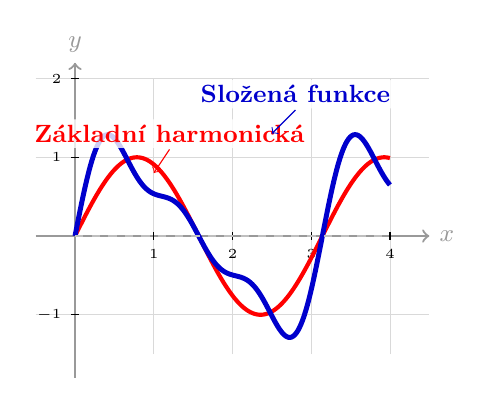
\begin{tikzpicture}[
        scale=1,
        axis/.style={->, thick, gray!80},
        function/.style={thick, smooth, samples=200},
        label/.style={font=\small}
    ]
    % Mřížka pro lepší orientaci
    \draw[gray!30, very thin] (-0.5,-1.5) grid (4.5,2);
    
    % Osy
    \draw[axis] (-0.5,0) -- (4.5,0) node[right, label] {$x$};
    \draw[axis] (0,-1.8) -- (0,2.2) node[above, label] {$y$};
    
    % Značky na osách
    \foreach \x in {1,2,3,4}
        \draw (\x,0.05) -- (\x,-0.05) node[below, font=\tiny] {$\x$};
    \foreach \y in {-1,1,2}
        \draw (0.05,\y) -- (-0.05,\y) node[left, font=\tiny] {$\y$};
    
    % Základní harmonická (červená)
    \draw[red, function, line width=1.5pt, domain=0:4] 
        plot (\x, {sin(2*\x r)});
    
    % Složená funkce (modrá)  
    \draw[blue!80!black, function, line width=1.8pt, domain=0:4] 
        plot (\x, {sin(2*\x r) + 0.4*sin(4*\x r) + 0.25*sin(6*\x r)});
    
    % Popisky s pozadím pro lepší čitelnost
    \node[red, font=\small\bfseries, 
          fill=white, fill opacity=0.8, text opacity=1,
          rounded corners=2pt, inner sep=2pt] 
        at (1.2,1.3) {Základní harmonická};
    
    \node[blue!80!black, font=\small\bfseries,
          fill=white, fill opacity=0.8, text opacity=1,
          rounded corners=2pt, inner sep=2pt] 
        at (2.8,1.8) {Složená funkce};
    
    % Šipky k funkcím
    \draw[->, red, thin] (1.2,1.1) -- (1,0.8);
    \draw[->, blue!80!black, thin] (2.8,1.6) -- (2.5,1.3);
    
    % Nulová linka
    \draw[gray!50, dashed, thin] (0,0) -- (4,0);
    
    \end{tikzpicture}
    \caption{Fourierova analýza: rozklad složené funkce na harmonické komponenty}
    \label{fig:fourier_decomposition}
    \end{figure}
    

\subsubsection{Projekční teorém a aplikace}

\begin{theorem}[Projekční teorém]
Nechť $H$ je Hilbertův prostor a $K \subset H$ uzavřený konvexní. Pak pro každé $x \in H$ existuje právě jedno $y \in K$ takové, že
\[
\|x - y\| = \inf_{z \in K} \|x - z\|
\]
\end{theorem}

\begin{keyinsight}
Rieszova věta umožňuje reprezentovat libovolný spojitý lineární funkcionál na Hilbertově prostoru pomocí skalárního součinu, což je fundamentální pro variační formulace diferenciálních rovnic.
\end{keyinsight}

\begin{example}[$L^2$ prostor a kvantové vlnové funkce]
V kvantové mechanice jsou vlnové funkce $\psi$ prvky $L^2(\mathbb{R}^3)$ s $\|\psi\|_2 = 1$. Skalární součin $\langle \psi, \phi \rangle$ má interpretaci amplitudy pravděpodobnosti přechodu mezi stavy.
\end{example}

\begin{application}
\begin{verbatim}
# Julia: Galerkinova projekce pro variační problémy
function galerkin_projection(basis_functions, bilinear_form, linear_form)
    n = length(basis_functions)
    A = zeros(n, n)
    b = zeros(n)
    for i in 1:n, j in 1:n
        A[i,j] = bilinear_form(basis_functions[i], basis_functions[j])
    end
    for i in 1:n
        b[i] = linear_form(basis_functions[i])
    end
    coefficients = A \ b
    return coefficients
end
\end{verbatim}
Projekční teorém zaručuje existenci nejlepší aproximace řešení v konečně-dimenzionálním podprostoru bázových funkcí. Ortogonální projekce minimalizuje chybu v energetické normě.
\end{application}

\begin{summary}
\textbf{Klíčové koncepty:} Skalární součin, ortogonalita, Fourierova řada. \\
\textbf{Hlavní výsledky:} Projekční teorém, Rieszova reprezentace. \\
\textbf{Aplikace:} Galerkinovy metody, kvantové vlnové funkce.
\end{summary}

\spc

\subsection{Lineární operátory a funkcionály}

\begin{scaffold}
\textbf{Co umíme:} Hilbertovy prostory a jejich geometrie z předchozí sekce. \\
\textbf{Co se naučíme:} Zobrazení mezi prostory a jejich spektrální vlastnosti. \\
\textbf{K čemu to využijeme:} Pro operátorový přístup k diferenciálním rovnicím a kvantovým systémům.
\end{scaffold}

\begin{motivation}
Diferenciální operátory jsou fundamentálním příkladem lineárních operátorů. Jejich vlastnosti určují existenci, jednoznačnost a kvalitativní chování řešení diferenciálních rovnic. V kvantové mechanice operátory reprezentují pozorovatelné veličiny.
\end{motivation}

\subsubsection{Základní třídy operátorů}

\begin{definition}[Lineární operátor]
Zobrazení $T: D(T) \subset X \to Y$ mezi vektorovými prostory je \emph{lineární}, jestliže
\[
T(\alpha x + \beta y) = \alpha T(x) + \beta T(y)
\]
\end{definition}

\begin{definition}[Ohraničený operátor]
Lineární operátor $T: X \to Y$ je \emph{ohraničený}, jestliže existuje $C > 0$ takové, že
\[
\|T(x)\|_Y \leq C \|x\|_X \quad \text{pro všechna } x \in X
\]
\end{definition}

\begin{example}[Derivační operátor]
Operátor $\frac{d}{dx}: C^1[0,1] \subset C[0,1] \to C[0,1]$ je lineární, ale není ohraničený v $\|\cdot\|_\infty$ normě, což vysvětluje citlivost diferenciálních rovnic na počáteční podmínky.
\end{example}

\begin{intuition}
Ohraničené operátory zachovávají konvergenci: $x_n \to x$ implikuje $T(x_n) \to T(x)$. Neohraničené operátory (jako derivace) tuto vlastnost postrádají, což koresponduje s možností chaotického chování v dynamických systémech.
\end{intuition}

\subsubsection{Duální prostory a geometrické principy}

\begin{definition}[Duální prostor]
Množina všech spojitých lineárních funkcionálů na $X$, značíme $X^*$.
\end{definition}

\begin{theorem}[Rieszova reprezentace]
Nechť $H$ je Hilbertův prostor. Pak pro každý $f \in H^*$ existuje právě jedno $y \in H$ takové, že
\[
f(x) = \langle x, y \rangle \quad \text{pro všechna } x \in H
\]
\end{theorem}

\begin{theorem}[Hahn-Banach]
Každý spojitý lineární funkcionál na podprostoru lze rozšířit na celý prostor bez zvýšení normy.
\end{theorem}

\begin{intuition}
Hahn-Banachova věta umožňuje "oddělit" bod od uzavřené konvexní množiny pomocí nadroviny. V optimalizaci: zaručuje existenci Lagrangeových multiplikátorů pro problémy s omezeními.
\end{intuition}

\begin{figure}[htbp]
    \centering
    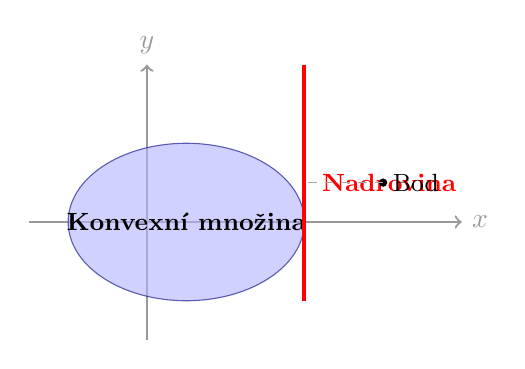
\begin{tikzpicture}[
    scale=1,
    axis/.style={->, thick, gray!80},
    set/.style={fill=blue!30, draw=blue!50!black, opacity=0.6},
    hyperplane/.style={red, line width=1.5pt},
    point/.style={fill=black, radius=1.5pt}
    ]
    % Osy pro kontext
    \draw[axis] (-1.5,0) -- (4,0) node[right] {$x$};
    \draw[axis] (0,-1.5) -- (0,2) node[above] {$y$};
    
    % Konvexní množina
    \draw[set] (0.5,0) ellipse (1.5 and 1);
    \node[font=\small\bfseries] at (0.5,0) {Konvexní množina};
    
    % Nadrovina
    \draw[hyperplane] (2,2) -- (2,-1);
    \node[red, font=\small\bfseries, anchor=west] at (2.1,0.5) {Nadrovina};
    
    % Bod a projekce
    \coordinate (P) at (3,0.5);
    \fill[point] (P) circle;
    \node[right, font=\small] at (P) {Bod};
    
    % Spojnice k nadrovině
    \draw[dashed, gray!70] (P) -- (2,0.5);
    
    \end{tikzpicture}
    \caption{Geometrická ilustrace konvexní množiny, nadroviny a bodu}
    \label{fig:convex_plane_point}
    \end{figure}

\subsubsection{Spektrální teorie - úvod}

\begin{definition}[Spektrální poloměr]
Pro ohraničený operátor $T$ definujeme
\[
r(T) = \sup\{|\lambda| : \lambda \in \sigma(T)\}
\]
\end{definition}

\begin{example}[Kvantový Hamiltonián]
Hamiltonián $\hat{H} = -\frac{\hbar^2}{2m}\nabla^2 + V(\mathbf{r})$ je neohraničený samosdružený operátor na $L^2(\mathbb{R}^3)$. Pro částici v nekonečné potenciálové jámě na $[0,L]$ má vlastní funkce $\psi_n(x) = \sqrt{\frac{2}{L}}\sin(\frac{n\pi x}{L})$ a vlastní hodnoty $E_n = \frac{n^2\pi^2\hbar^2}{2mL^2}$.
\end{example}

\begin{keyinsight}
Spektrální vlastnosti lineárních operátorů určují stabilitu řešení ODR a energetické hladiny kvantových systémů. Samosdruženost operátorů zajišťuje realitu spektra, což je fyzikálně nezbytné pro interpretaci vlastních hodnot jako měřitelných veličin.
\end{keyinsight}

\begin{application}
V analýze stability ODR: Spektrum linearizovaného operátoru určuje stabilitu rovnovážných bodů. V kvantové mechanice: spektrum Hamiltoniánu určuje možné energetické stavy systému.
\end{application}

\begin{summary}
\textbf{Klíčové koncepty:} Lineární operátor, duální prostor, spektrum. \\
\textbf{Hlavní výsledky:} Rieszova reprezentace, Hahn-Banachova věta. \\
\textbf{Aplikace:} Kvantové Hamiltoniány, stabilita dynamických systémů.
\end{summary}

\spc

\subsection{Teorie míry a Lebesgueův integrál}

\begin{scaffold}
\textbf{Co umíme:} Základy funkcionální analýzy z předchozích sekcí. \\
\textbf{Co se naučíme:} Moderní teorie integrace a míry. \\
\textbf{K čemu to využijeme:} Pro práci s $L^p$ prostory a slabou formulaci diferenciálních rovnic.
\end{scaffold}

\begin{motivation}
Lebesgueův integrál poskytuje mocný aparát pro práci s funkcemi, které nejsou spojité, a je základem moderní analýzy a teorie pravděpodobnosti. Bez něj bychom nemohli rigorózně definovat prostory $L^p$ potřebné pro slabou formulaci ODR/PDR.
\end{motivation}

\subsubsection{Základní pojmy teorie míry}

\begin{definition}[$\sigma$-algebra]
Množina $\mathcal{A}$ podmnožin $X$ je \emph{$\sigma$-algebra}, jestliže:
\begin{enumerate}
\item $X \in \mathcal{A}$
\item $A \in \mathcal{A} \Rightarrow A^c \in \mathcal{A}$
\item $A_n \in \mathcal{A} \Rightarrow \bigcup_{n=1}^\infty A_n \in \mathcal{A}$
\end{enumerate}
\end{definition}

\begin{definition}[Míra]
Funkce $\mu: \mathcal{A} \to [0,\infty]$ je \emph{míra}, jestliže:
\begin{enumerate}
\item $\mu(\emptyset) = 0$
\item $\mu\left(\bigcup_{n=1}^\infty A_n\right) = \sum_{n=1}^\infty \mu(A_n)$ pro disjunktní $A_n$
\end{enumerate}
\end{definition}

\begin{intuition}
$\sigma$-algebra představuje množinu "měřitelných" množin. Míra přiřazuje každé měřitelné množině její "velikost". Lebesgueova míra zobecňuje pojem délky/obsahu/objemu na širší třídu množin.
\end{intuition}

\subsubsection{Lebesgueův integrál a konvergenční věty}

\begin{definition}[Měřitelná funkce]
Funkce $f: X \to \mathbb{R}$ je \emph{měřitelná}, jestliže $f^{-1}((a,\infty)) \in \mathcal{A}$ pro všechna $a \in \mathbb{R}$.
\end{definition}

\begin{theorem}[Konvergenční věty]
\begin{itemize}
\item \emph{Monotónní konvergence}: Jestliže $0 \leq f_n \nearrow f$, pak $\int f_n \, d\mu \nearrow \int f \, d\mu$
\item \emph{Dominovaná konvergence}: Jestliže $f_n \to f$ a $|f_n| \leq g$ integrovatelná, pak $\int f_n \, d\mu \to \int f \, d\mu$
\end{itemize}
\end{theorem}

\begin{intuition}
Lebesgueův integrál měří "plochu pod grafem" horizontálním řezáním podle funkčních hodnot, na rozdíl od Riemannova vertikálního řezání podle definičního oboru. Konvergenční věty zásadně rozšiřují možnosti analýzy tím, že umožňují záměnu limity a integrálu za velmi obecných podmínek.
\end{intuition}

\begin{theorem}[Radon-Nikodym]
Nechť $\mu$ a $\nu$ jsou $\sigma$-konečné míry na $(X,\mathcal{A})$ a $\nu \ll \mu$. Pak existuje měřitelná funkce $f: X \to [0,\infty)$ taková, že
\[
\nu(A) = \int_A f \, d\mu \quad \text{pro všechna } A \in \mathcal{A}
\]
\end{theorem}

\begin{keyinsight}
Radon-Nikodymova věta umožňuje transformovat jednu míru na druhou pomocí derivace míry, což je fundamentální pro teorii pravděpodobnosti a stochastické analýzu.
\end{keyinsight}

\subsubsection{$L^p$ prostory a jejich vlastnosti}

\begin{definition}[$L^p$ prostor]
\[
L^p(\Omega) = \left\{ f: \Omega \to \mathbb{C} \text{ měřitelné} : \int_\Omega |f|^p \, d\mu < \infty \right\}
\]
s normou $\|f\|_p = \left(\int_\Omega |f|^p \, d\mu\right)^{1/p}$
\end{definition}

\begin{theorem}[Riesz-Fischer]
$L^p$ prostory jsou úplné pro $1 \leq p \leq \infty$.
\end{theorem}

\begin{keyinsight}
$L^2$ prostor je Hilbertův prostor, $L^1$ a $L^\infty$ jsou Banachovy prostory. $L^p$ prostory tvoří přirozený rámec pro slabá řešení ODR i PDR - funkce v $W^{1,2}(a,b)$ jsou přirozeným prostorem pro slabá řešení ODR druhého řádu, kde klasické derivace jsou nahrazeny zobecněnými derivacemi.
\end{keyinsight}

\begin{application}
V modelování Brownova pohybu: Trajektorie Brownova pohybu jsou s pravděpodobností 1 nespojité a nikde diferencovatelné, ale měřitelné funkce, což vyžaduje Lebesgueův integrál pro jejich analýzu. $L^2$ prostor je navíc přirozeným prostředím pro stochastické integrály.
\end{application}

\begin{summary}
\textbf{Klíčové koncepty:} $\sigma$-algebra, míra, měřitelná funkce, $L^p$ prostory. \\
\textbf{Hlavní výsledky:} Konvergenční věty, Radon-Nikodymova věta, Riesz-Fischer. \\
\textbf{Aplikace:} Brownův pohyb, slabá formulace ODR/PDR.
\end{summary}

\spc

\subsection{Sobolevovy prostory}

\begin{scaffold}
\textbf{Co umíme:} $L^p$ prostory a Lebesgueův integrál z předchozí sekce. \\
\textbf{Co se naučíme:} Prostory funkcí se zobecněnými derivacemi. \\
\textbf{K čemu to využijeme:} Pro formulaci a analýzu slabých řešení ODR/PDR.
\end{scaffold}

\begin{motivation}
Sobolevovy prostory přirozeně zachycují regularitu řešení diferenciálních rovnic prostřednictvím zobecněných derivací a jsou klíčové pro slabou formulaci. Umožňují pracovat s řešeními, která nejsou dostatečně hladká pro klasickou interpretaci, ale stále mají "derivaci v průměru".
\end{motivation}

\subsubsection{Zobecněné derivace}

\begin{definition}[Slabá derivace]
Funkce $v \in L^1_{\text{loc}}(\Omega)$ je \emph{slabou derivací} $u$ v multiindexu $\alpha$, jestliže
\[
\int_\Omega u D^\alpha \phi \, dx = (-1)^{|\alpha|} \int_\Omega v \phi \, dx \quad \text{pro všechny } \phi \in C_c^\infty(\Omega)
\]
\end{definition}

\begin{intuition}
Slabá derivace zobecňuje klasickou derivaci pomocí "integrace per partes". Umožňuje derivovat funkce, které nejsou hladké, ale stále mají "derivaci v průměru". Tato myšlenka je fundamentální pro moderní teorii parciálních diferenciálních rovnic.
\end{intuition}

\subsubsection{Sobolevovy prostory a vnořovací věty}

\begin{definition}[Sobolevův prostor]
\[
W^{k,p}(\Omega) = \{ u \in L^p(\Omega) : D^\alpha u \in L^p(\Omega) \text{ pro } |\alpha| \leq k \}
\]
s normou $\|u\|_{k,p} = \left( \sum_{|\alpha| \leq k} \|D^\alpha u\|_p^p \right)^{1/p}$
\end{definition}

\begin{theorem}[Vnořovací věty]
\begin{itemize}
\item \emph{Sobolev}: $W^{k,p}(\Omega) \hookrightarrow L^q(\Omega)$ pro vhodné $q$
\item \emph{Rellich-Kondrachov}: $W^{k,p}(\Omega) \hookrightarrow\hookrightarrow L^p(\Omega)$ je kompaktní vnoření
\end{itemize}
\end{theorem}

\begin{keyinsight}
Sobolevovy vnořovací věty určují regularitu řešení diferenciálních rovnic. Například pro ODR druhého řádu: řešení v $W^{2,p}$ jsou spojitá pro $p$ dostatečně velké. Kompaktní vnoření zaručuje konvergenci podposloupností, což je klíčové pro důkazy existence řešení variačními metodami.
\end{keyinsight}

\begin{figure}[htbp]
    \centering
    \begin{tikzpicture}[
        scale=1,
        axis/.style={->, thick, black},
        space/.style={font=\small\bfseries},
        inc/.style={-Stealth, thick, blue}
    ]
    % Osy
    \draw[axis] (0,0) -- (4.5,0) node[right] {Regularita};
    \draw[axis] (0,0) -- (0,3.5) node[above] {Prostor};
    
    % Prostory
    \node[space] (C) at (1,0.5) {$C[a,b]$};
    \node[space] (Lp) at (2,1.2) {$L^p(a,b)$};
    \node[space] (W) at (3,2.5) {$W^{1,p}(a,b)$};
    
    % Šipky inkluzí
    \draw[inc] (C.north east) -- (Lp.south west) node[midway, above, sloped] {kontinuální};
    \draw[inc] (Lp.north east) -- (W.south west) node[midway, above, sloped] {kompaktní};
    
    \end{tikzpicture}
    \caption{Hierarchie funkcí v prostorech $C[a,b]\subset L^p(a,b)\subset W^{1,p}(a,b)$.}
    \label{fig:prostorova-hierarchie}
\end{figure}
        

\subsubsection{Trakce a aplikace}

\begin{definition}[Trakce]
Pro $u \in W^{1,p}(\Omega)$ existuje zobrazení $\gamma: W^{1,p}(\Omega) \to L^p(\partial\Omega)$ takové, že $\gamma(u) = u|_{\partial\Omega}$ pro $u \in C(\overline{\Omega})$.
\end{definition}

\begin{intuition}
Trakce umožňuje smysluplně definovat okrajové hodnoty i pro funkce, které nejsou spojité - klíčové pro formulaci okrajových úloh. I když funkce z $W^{1,p}$ nemusí být spojité, jejich "stopa" na hranici je dobře definována.
\end{intuition}

\begin{application}
Ve Finite Element Method: Sobolevovy prostory poskytují teoretický základ pro analýzu konvergence a odhadů chyb numerických aproximací. Galerkinova metoda hledá aproximace řešení v konečně-dimenzionálních podprostorech Sobolevových prostorů.
\end{application}

\begin{summary}
\textbf{Klíčové koncepty:} Slabá derivace, Sobolevův prostor, trakce. \\
\textbf{Hlavní výsledky:} Vnořovací věty (Sobolev, Rellich-Kondrachov). \\
\textbf{Aplikace:} Slabá formulace ODR/PDR, FEM.
\end{summary}

\spc

\subsection{Základy spektrální teorie}

\begin{scaffold}
\textbf{Co umíme:} Lineární operátory a funkcionály z předchozích sekcí. \\
\textbf{Co se naučíme:} Spektrum operátorů a jejich rozklad na vlastní složky. \\
\textbf{K čemu to využijeme:} Pro analýzu kvantových Hamiltoniánů a stability dynamických systémů.
\end{scaffold}

\begin{motivation}
Spektrální teorie umožňuje analyzovat lineární operátory pomocí jejich vlastních hodnot a vektorů - fundamentální nástroj pro kvantovou mechaniku a stabilitu dynamických systémů. Spektrální rozklad operátoru je analogický diagonalizaci matice v lineární algebře.
\end{motivation}

\subsubsection{Základní pojmy spektrální teorie}

\begin{definition}[Spektrum operátoru]
Pro operátor $T: D(T) \subset X \to X$ definujeme:
\begin{itemize}
\item \emph{Bodové spektrum}: $\sigma_p(T) = \{\lambda : T - \lambda I \text{ není prosté}\}$
\item \emph{Spojité spektrum}: $\sigma_c(T) = \{\lambda : T - \lambda I \text{ je prosté, ale nemá uzavřený obor hodnot}\}$
\item \emph{Reziduální spektrum}: $\sigma_r(T) = \{\lambda : T - \lambda I \text{ je prosté, ale obor hodnot není hustý}\}$
\end{itemize}
\end{definition}

\begin{intuition}
Spektrum operátoru zobecňuje pojem vlastních čísel matice. Bodové spektrum odpovídá vlastním hodnotám, spojité spektrum vzniká v nekonečné dimenzi a odpovídá "spojitému" rozložení možných měření v kvantové mechanice.
\end{intuition}

\subsubsection{Kompaktní operátory a jejich spektrum}

\begin{definition}[Kompaktní operátor]
Operátor $T: X \to Y$ je \emph{kompaktní}, jestliže zobrazuje ohraničené množiny na relativně kompaktní.
\end{definition}

\begin{theorem}[Spektrum kompaktního operátoru]
Nechť $T$ je kompaktní operátor na Banachově prostoru. Pak:
\begin{itemize}
\item $0 \in \sigma(T)$
\item $\sigma(T) \setminus \{0\}$ se skládá z vlastních čísel konečné multiplicity
\item Mohou se hromadit pouze v nule
\end{itemize}
\end{theorem}

\begin{intuition}
Spektrální rozklad kompaktního operátoru zásadně rozšiřuje možnosti analýzy tím, že umožňuje reprezentovat operátor jako součet jednodušších komponent, analogicky k diagonálnímu tvaru matice v konečné dimenzi.
\end{intuition}

\begin{example}[Spektrální rozklad integrálního operátoru]
Uvažujme operátor $T: L^2[0,1] \to L^2[0,1]$ definovaný jako
\[
(Tf)(x) = \int_0^1 K(x,y)f(y)dy
\]
kde $K(x,y) = \min(x,y) - xy$. Tento operátor má vlastní funkce $\phi_n(x) = \sqrt{2}\sin(n\pi x)$ a vlastní čísla $\lambda_n = \frac{1}{n^2\pi^2}$. Spektrální rozklad má tvar:
\[
Tf = \sum_{n=1}^\infty \frac{1}{n^2\pi^2} \langle f, \phi_n \rangle \phi_n
\]
\end{example}

\subsubsection{Samosdružené operátory v kvantové mechanice}

\begin{definition}[Samosdružený operátor]
Operátor $T$ na Hilbertově prostoru je \emph{samosdružený}, jestliže $T = T^*$.
\end{definition}

\begin{theorem}[Vlastnosti samosdružených operátorů]
\begin{itemize}
\item Spektrum je reálné
\item Vlastní vektory příslušné různým vlastním číslům jsou ortogonální
\item Existuje spektrální rozklad
\end{itemize}
\end{theorem}

\begin{example}[Kvantový Hamiltonián]
V kvantové mechanice je Hamiltonián $\hat{H} = -\frac{\hbar^2}{2m}\nabla^2 + V(\mathbf{r})$ samosdružený operátor na $L^2(\mathbb{R}^3)$. Pro částici v nekonečné potenciálové jámě na $[0,L]$ má vlastní funkce $\psi_n(x) = \sqrt{\frac{2}{L}}\sin(\frac{n\pi x}{L})$ a vlastní hodnoty $E_n = \frac{n^2\pi^2\hbar^2}{2mL^2}$. Spektrální rozklad:
\[
\hat{H}\psi = \sum_{n=1}^\infty E_n \langle \psi, \psi_n \rangle \psi_n
\]
\end{example}

\begin{keyinsight}
Samosdruženost kvantových operátorů zajišťuje realitu spektra (energií) a unitární evoluci (zachování pravděpodobnosti). Spektrální teorém pro samosdružené operátory je matematickým základem kvantové mechaniky - vlastní hodnoty představují možné výsledky měření, vlastní funkce odpovídají stavům s definovanou hodnotou dané veličiny.
\end{keyinsight}

\begin{application}
V analýze stability ODR: Spektrum linearizovaného operátoru určuje stabilitu rovnovážných bodů dynamických systémů. V kvantové mechanice: spektrum Hamiltoniánu určuje možné energetické stavy systému a spektrální rozklad umožňuje vývoj kvantového stavu v čase.
\end{application}

\begin{summary}
\textbf{Klíčové koncepty:} Spektrum, kompaktní operátor, samosdruženost. \\
\textbf{Hlavní výsledky:} Spektrum kompaktních operátorů, spektrální rozklad. \\
\textbf{Aplikace:} Kvantové Hamiltoniány, stabilita dynamických systémů.
\end{summary}

\spc

\subsection{Teorie distribucí (úvod)}

\begin{scaffold}
\textbf{Co umíme:} Sobolevovy prostory a slabé derivace z předchozí sekce. \\
\textbf{Co se naučíme:} Zobecněné funkce a operace s nimi. \\
\textbf{K čemu to využijeme:} Pro slabou formulaci diferenciálních rovnic a teorii fundamentálních řešení.
\end{scaffold}

\begin{motivation}
Distribuce zobecňují pojem funkce a umožňují smysluplně derivovat i velmi nepravidelné objekty - klíčové pro slabou formulaci diferenciálních rovnic. Umožňují pracovat s matematickými objekty jako je Diracova delta, které nemají klasickou interpretaci, ale mají hluboký fyzikální význam jako modely impulzních reakcí v reálných experimentech.
\end{motivation}

\subsubsection{Základní definice a příklady}

\begin{definition}[Prostor testovacích funkcí]
$C_c^\infty(\Omega)$ s topologií konvergence: $\phi_n \to \phi$ jestliže existuje kompakt $K$ s $\supp \phi_n \subset K$ a $D^\alpha \phi_n \to D^\alpha \phi$ stejnoměrně.
\end{definition}

\begin{definition}[Distribuce]
Lineární funkcionál $T: C_c^\infty(\Omega) \to \mathbb{C}$, který je spojitý v uvedené topologii.
\end{definition}

\begin{example}[Základní distribuce]
\begin{itemize}
\item \emph{Regularní distribuce}: $T_f(\phi) = \int_\Omega f\phi \, dx$ pro $f \in L^1_{\text{loc}}$
\item \emph{Diracova delta}: $\delta(\phi) = \phi(0)$
\item \emph{Cauchyho hlavní hodnota}: $\mathrm{p.v.}\frac{1}{x}(\phi) = \lim_{\epsilon \to 0} \int_{|x|>\epsilon} \frac{\phi(x)}{x} \, dx$
\end{itemize}
\end{example}

\begin{intuition}
Distribuce nelze hodnotit v bodech, ale pouze "testovat" proti hladkým funkcím. Diracova delta $\delta$ se chová jako "funkce", která je nulová všude kromě nuly, kde je nekonečná, ale její integrál je 1. Tento zdánlivě paradoxní objekt má přirozenou interpretaci jako jednotkový impuls v teorii signálů a fyzikálních modelech.
\end{intuition}

\subsubsection{Operace s distribucemi a fyzikální interpretace}

\begin{definition}[Derivace distribuce]
$T'(\phi) = -T(\phi')$
\end{definition}

\begin{definition}[Konvoluce distribucí]
Pro distribuci $T$ a testovací funkci $\phi$ definujeme konvoluci $T * \phi$ jako funkci
\[
(T * \phi)(x) = T(\phi(x - \cdot))
\]
Pro distribuci $T$ a funkci $\psi$ definujeme konvoluci $T * \psi$ jako distribuci
\[
(T * \psi)(\phi) = T(\psi * \phi)
\]
\end{definition}

\begin{intuition}
Konvoluce distribuce s testovací funkcí funguje jako "vyhlazování". Fyzikální analogie: Diracova delta představuje jednotkový impuls, konvoluce $\delta * f$ dává odezvu lineárního systému na tento impuls. Tento princip je základem teorie Greenových funkcí v diferenciálních rovnicích a modeluje impulzní reakce v reálných experimentech.
\[
\text{Impuls } \delta \rightarrow [\text{Lineární systém } L] \rightarrow \text{Odezva } G
\]
kde $G$ je Greenova funkce splňující $LG = \delta$.
\end{intuition}

\begin{definition}[Konvergence distribucí]
$T_n \to T$ jestliže $T_n(\phi) \to T(\phi)$ pro všechny testovací funkce $\phi$.
\end{definition}

\begin{example}[Aproximace Diracovy delta]
Posloupnost funkcí $\delta_n(x) = \frac{n}{\sqrt{\pi}} e^{-(nx)^2}$ konverguje k $\delta$ v distribucích, neboť pro každou testovací funkci $\phi$ platí:
\[
\lim_{n\to\infty} \int_{-\infty}^\infty \delta_n(x)\phi(x)dx = \phi(0)
\]
\end{example}

\begin{keyinsight}
Teorie distribucí umožňuje pracovat s derivacemi funkcí, které klasicky derivovatelné nejsou, a poskytuje přirozený rámec pro fundamentální řešení diferenciálních operátorů. Distribuce tvoří duální prostor k prostoru testovacích funkcí a tato dualita je základem slabé formulace diferenciálních rovnic.
\end{keyinsight}

\begin{application}
V teorii parciálních diferenciálních rovnic: Fundamentální řešení je distribuce, která řeší rovnici $Lu = \delta$, kde $L$ je diferenciální operátor. Greenova funkce pak umožňuje vyjádřit řešení nehomogenní rovnice jako konvoluci s pravou stranou. V elektromagnetismu: Diracova delta modeluje bodové náboje, v mechanice bodové síly.
\end{application}

\begin{summary}
\textbf{Klíčové koncepty:} Testovací funkce, distribuce, slabá derivace, konvoluce. \\
\textbf{Hlavní výsledky:} Operace s distribucemi, konvergence distribucí. \\
\textbf{Aplikace:} Greenovy funkce, fundamentální řešení, impulzní reakce.
\end{summary}

\spc

\subsection*{Shrnutí kapitoly}

\begin{itemize}
\item Vybudován logický aparát metrických, normovaných a Hilbertových prostorů jako prostředí pro analýzu diferenciálních rovnic

\item Představen operátorový přístup s důrazem na spektrální vlastnosti lineárních operátorů a jejich aplikace v kvantové mechanice

\item Zaveden Lebesgueův integrál a $L^p$ prostory jako základ moderní funkcionální analýzy a teorie pravděpodobnosti

\item Definovány Sobolevovy prostory zachycující regularitu řešení prostřednictvím zobecněných derivací - přirozené prostředí pro slabá řešení ODR/PDR

\item Uvedena spektrální teorie jako matematický základ kvantové mechaniky s explicitními příklady spektrálních rozkladů

\item Připraven úvod do teorie distribucí pro následující kapitoly o slabých řešeních a Greenových funkcích
\end{itemize}

\begin{literature}
\textbf{Doporučená literatura pro hlubší studium:}
\begin{itemize}
\item Evans, L. C. \emph{Partial Differential Equations} (GSM 19)
\item Brezis, H. \emph{Functional Analysis, Sobolev Spaces and Partial Differential Equations}
\item Reed, M.; Simon, B. \emph{Methods of Modern Mathematical Physics I: Functional Analysis}
\item Rudin, W. \emph{Real and Complex Analysis}
\end{itemize}
\end{literature}

\begin{transition}
V \hyperref[sec:zakladni-teoremy]{Kapitole 3} aplikujeme tento matematický aparát na základní teorémy existence a jednoznačnosti řešení obyčejných diferenciálních rovnic. Konkrétně využijeme Banachovy prostory pro Picardovu iteraci, Sobolevovy prostory pro slabou formulaci a spektrální teorii pro analýzu stability řešení.
\end{transition}

\spc